\documentclass[usenames,dvipsnames]{beamer}
\usetheme{Boadilla}
\usecolortheme{default}
% \usepackage{pgfpages} % TO DELETE
% \setbeameroption{hide notes} % Only slides
% \setbeameroption{show only notes} % Only notes
\setbeameroption{show notes on second screen=right} % Both
\setbeamertemplate{note page}{\pagecolor{yellow!5}\insertnote}\usepackage{palatino}

\usepackage[utf8]{inputenc}
\usepackage[round]{natbib}
\renewcommand*{\bibfont}{\scriptsize}
\usepackage{tikz}


\DeclareMathOperator{\rank}{rank}
\DeclareMathOperator{\erank}{erank}
\DeclareMathOperator{\cl}{cl}
\DeclareMathOperator{\diag}{diag}
\DeclareMathOperator{\spn}{span}
% \newtheorem{theorem}{Theorem}
\newtheorem{assumption}{Assumption}
% \newtheorem{definition}{Definition}
\newtheorem{observation}{Observation}
% \newtheorem{corollary}{Corollary}
% \newtheorem{lemma}{Lemma}
\usepackage{dsfont}
\newcommand{\onefunc}{\mathds{1}}
\newcommand{\din}{{d_{\text{in}}}}
\newcommand{\dhid}{{d_{\text{hidden}}}}
\newcommand{\dout}{{d_{\text{out}}}}
\newcommand{\eps}{\epsilon}
\newcommand{\TODO}{\Red{TODO}}
\newcommand{\abs}[1]{\left|{#1}\right|}
\newcommand{\tr}[1]{\text{Tr}\left({#1}\right)}
\newcommand{\vect}[1]{\text{vec}\left({#1}\right)}
\newcommand{\opt}[1]{#1^\star}
\newcommand{\norm}[2][]{{\left\|{#2}\right\|_{#1}}}
%\newcommand{\norm}[1]{\left\|#1\right\|}
\newcommand{\snorm}[1]{\|#1\|} %small norm
\renewcommand{\angle}[2]{\measuredangle \left( #1, #2 \right)}
\newcommand{\bigangle}[2]{\measuredangle \left\big( #1, #2 \right\big)}
\newcommand{\Red}[1]{\colorbox{red}{#1}}
\newcommand{\set}[1]{\left\{{#1}\right\}}

\newcommand{\ba}{\mathbf{a}}
\newcommand{\be}{\mathbf{e}}
\newcommand{\bx}{\mathbf{x}}
\newcommand{\bw}{\mathbf{w}}
\newcommand{\bg}{\mathbf{g}}
\newcommand{\bb}{\mathbf{b}}
\newcommand{\bu}{\mathbf{u}}
\newcommand{\bv}{\mathbf{v}}
\newcommand{\bz}{\mathbf{z}}
\newcommand{\bc}{\mathbf{c}}
\newcommand{\br}{\mathbf{r}}
\newcommand{\bd}{\mathbf{d}}
\newcommand{\bp}{\mathbf{p}}
\newcommand{\bh}{\mathbf{h}}
\newcommand{\by}{\mathbf{y}}
\newcommand{\bn}{\mathbf{n}}
\newcommand{\bs}{\mathbf{s}}
\newcommand{\bq}{\mathbf{q}}
\newcommand{\bmu}{\boldsymbol{\mu}}
\newcommand{\balpha}{\boldsymbol{\alpha}}
\newcommand{\bbeta}{\boldsymbol{\beta}}
\newcommand{\btau}{\boldsymbol{\tau}}
\newcommand{\bxi}{\boldsymbol{\xi}}
\newcommand{\blambda}{\boldsymbol{\lambda}}
\newcommand{\bepsilon}{\boldsymbol{\epsilon}}
\newcommand{\bsigma}{\boldsymbol{\sigma}}
\newcommand{\btheta}{{\boldsymbol{\theta}}}
\newcommand{\bomega}{\boldsymbol{\omega}}
\newcommand{\Xcal}{\mathcal{X}}

\newcommand{\co}{{\cal O}}
\newcommand{\ca}{{\cal A}}
\newcommand{\cb}{{\cal B}}
\newcommand{\cd}{{\cal D}}
\newcommand{\cdb}{{\cal D}^{\rm b}}
\newcommand{\cc}{{\cal C}}
\newcommand{\ck}{{\cal K}}
\newcommand{\cq}{{\cal Q}}
\newcommand{\ce}{{\cal E}}
\newcommand{\ct}{{\cal T}}
\newcommand{\cg}{{\cal G}}
\newcommand{\ch}{{\cal H}}
\newcommand{\cm}{{\cal M}}
\newcommand{\ci}{{\cal I}}
\newcommand{\cj}{{\cal J}}
\newcommand{\cw}{{\cal W}}
%\newcommand{\cl}{{\cal L}}
\newcommand{\cf}{{\cal F}}
\newcommand{\cv}{{\cal V}}
\newcommand{\cp}{{\cal P}}
\newcommand{\cu}{{\cal U}}
\newcommand{\cx}{{\cal X}}
\newcommand{\cy}{{\cal Y}}
\newcommand{\cz}{{\cal Z}}
\newcommand{\cs}{{\cal S}}
\newcommand{\cn}{{\cal N}}
\newcommand{\calr}{{\cal R}}

\newcommand{\bbs}{{\mathbb S}}
\newcommand{\reals}{{\mathbb R}}
\newcommand{\nat}{{\mathbb N}}
\newcommand{\integers}{{\mathbb Z}}
\newcommand{\complex}{{\mathbb C}}
\newcommand{\zero}{{\mathbf{0}}}

% Style conventions
\newcommand{\true}[1]{{\textcolor{ForestGreen}{\textbf{#1}}}}




\title[Implicit Reg.: Rank Min. in ReLU Networks]{Implicit Regularization Towards Rank Minimization in ReLU Networks}
\author[Nadav Timor]{
    by Nadav Timor\newline
    Advisor: Prof. Ohad Shamir
}
\institute[Weizmann Institute]{Weizmann Institute of Science}
\date[January 2022]{January 2022}
% \logo{
\includegraphics[height=.75cm]{WeizmannLogo.png}}



\begin{document}



\frame{\titlepage}

\begin{frame}
    \frametitle{Implicit~Regularization Towards Rank~Minimization\\in ReLU~Networks}
    A joint paper under review @ ICML 2022,\\
    w/ Gal Vardi and Ohad Shamir.
\end{frame}



\section{What is implicit regularization?}

\begin{frame}{What is \emph{implicit regularization}?}{How to generalize despite overparameterization?}
    \pause
    \newline
    If \#[learnable parameters] $>>$ \#[training examples]:
    \pause
    \begin{columns}
        \column{0.5\textwidth}
        \begin{itemize}
            \item \alert{Many global minima}\\
            (w/ $0$ training loss).
            \pause
            \item Might \alert{overfit}.
            \pause
            \begin{itemize}
                \item Popular solution:\\\true{explicit regularization}.
            \end{itemize}
        \end{itemize}
        \column{0.5\textwidth}
        \begin{figure}
        \centering
            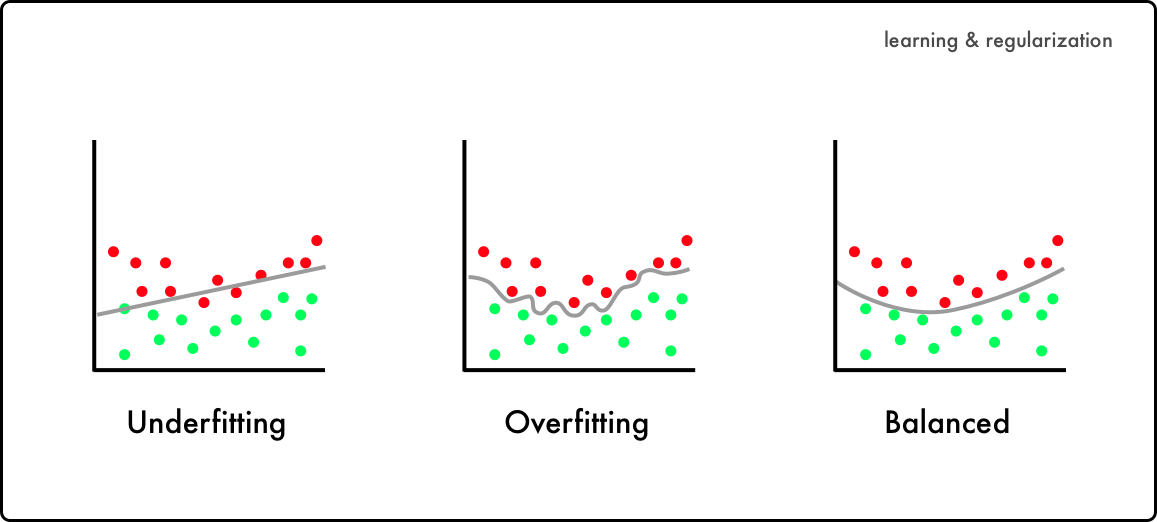
\includegraphics[width=6cm]{figures/overfitting.png}
            % \caption{}
            % \label{fig:overfitting}
        \end{figure}
    \end{columns}
    \pause
    \begin{block}{Phenomenon in practice (\cite{zhang2017understanding})}
        Networks trained \alert{w/o explicit~regularization} \true{generalize well}.
        \newline
        \newline
        (despite \#[learnable parameters] $>>$ \#[training examples])
    \end{block}
    \pause
    \textbf{Q:} How?\\
    \pause
    \textbf{Possible A:} ``implicit regularization'' (or ``implicit bias'').
    
    \note{
        \alert{If asked:}
        \begin{enumerate}
            \item \cite{zhang2017understanding}:\\
            Large CNNs, trained w/ stochastic~gradient~methods\\
            fit a random~labeling (of the training~data), or even completely~unstructured random~noise.\\
            Unaffected by explicit~regularization.
        \end{enumerate}
    }
\end{frame}




\begin{frame}{What is \emph{implicit regularization}?}
    \tikzset{every picture/.style={line width=0.75pt}} %set default line width to 0.75pt        
    
    \begin{tikzpicture}[x=0.75pt,y=0.75pt,yscale=-1,xscale=1]
        % uncomment if require: \path (0,261); %set diagram left start at 0, and has height of 261
        
        % 1. theta(0) := initial parameterization
        %Shape: Ellipse [id:dp021475373846624457] 
        \draw  [fill={rgb, 255:red, 148; green, 196; blue, 242 }  ,fill opacity=0.48 ] (6,128.75) .. controls (6,60.96) and (108.97,6) .. (236,6) .. controls (363.03,6) and (466,60.96) .. (466,128.75) .. controls (466,196.54) and (363.03,251.5) .. (236,251.5) .. controls (108.97,251.5) and (6,196.54) .. (6,128.75) -- cycle ;
        % Text Node
        \draw (109,24) node [anchor=north west][inner sep=0.75pt]  [font=\Large] [align=left] {$\displaystyle \mathbb{R}^{d}$};
        % Text Node
        \draw (338,28) node [anchor=north west][inner sep=0.75pt]  [font=\small] [align=left] {$\displaystyle \boldsymbol{\theta }(\boldsymbol{0})$};
        % Text Node
        \draw (377,46) node [anchor=north west][inner sep=0.75pt]  [font=\small] [align=left] {$\displaystyle \boldsymbol{\theta }(\boldsymbol{0})$};
        % Text Node
        \draw (405,64) node [anchor=north west][inner sep=0.75pt]  [font=\small] [align=left] {$\displaystyle \boldsymbol{\theta }(\boldsymbol{0})$};
        % Text Node
        \draw (426,89) node [anchor=north west][inner sep=0.75pt]  [font=\small] [align=left] {$\displaystyle \boldsymbol{\theta }(\boldsymbol{0})$};
        %Shape: Circle [id:dp6052897788269528] 
        \draw  [fill={rgb, 255:red, 0; green, 0; blue, 0 }  ,fill opacity=1 ] (343,44.5) .. controls (343,42.71) and (344.46,41.25) .. (346.25,41.25) .. controls (348.04,41.25) and (349.5,42.71) .. (349.5,44.5) .. controls (349.5,46.29) and (348.04,47.75) .. (346.25,47.75) .. controls (344.46,47.75) and (343,46.29) .. (343,44.5) -- cycle ;
        %Shape: Circle [id:dp38777159033159503] 
        \draw  [fill={rgb, 255:red, 0; green, 0; blue, 0 }  ,fill opacity=1 ] (383,62.5) .. controls (383,60.71) and (384.46,59.25) .. (386.25,59.25) .. controls (388.04,59.25) and (389.5,60.71) .. (389.5,62.5) .. controls (389.5,64.29) and (388.04,65.75) .. (386.25,65.75) .. controls (384.46,65.75) and (383,64.29) .. (383,62.5) -- cycle ;
        %Shape: Circle [id:dp2748850897412932] 
        \draw  [fill={rgb, 255:red, 0; green, 0; blue, 0 }  ,fill opacity=1 ] (411,80.5) .. controls (411,78.71) and (412.46,77.25) .. (414.25,77.25) .. controls (416.04,77.25) and (417.5,78.71) .. (417.5,80.5) .. controls (417.5,82.29) and (416.04,83.75) .. (414.25,83.75) .. controls (412.46,83.75) and (411,82.29) .. (411,80.5) -- cycle ;
        %Shape: Circle [id:dp7882824625742048] 
        \draw  [fill={rgb, 255:red, 0; green, 0; blue, 0 }  ,fill opacity=1 ] (432,105.5) .. controls (432,103.71) and (433.46,102.25) .. (435.25,102.25) .. controls (437.04,102.25) and (438.5,103.71) .. (438.5,105.5) .. controls (438.5,107.29) and (437.04,108.75) .. (435.25,108.75) .. controls (433.46,108.75) and (432,107.29) .. (432,105.5) -- cycle ;
        
        % 2. GF guarantee convergence to a local min.
        \pause
        %Shape: Ellipse [id:dp1447748006695847] 
        \draw  [fill={rgb, 255:red, 148; green, 180; blue, 242 }  ,fill opacity=0.5 ] (54,148) .. controls (54,100.23) and (140.86,61.5) .. (248,61.5) .. controls (355.14,61.5) and (442,100.23) .. (442,148) .. controls (442,195.77) and (355.14,234.5) .. (248,234.5) .. controls (140.86,234.5) and (54,195.77) .. (54,148) -- cycle ;
        %Shape: Ellipse [id:dp8297282672351468] 
        \draw  [fill={rgb, 255:red, 148; green, 160; blue, 242 }  ,fill opacity=0.61 ] (133,169) .. controls (133,138.9) and (191.87,114.5) .. (264.5,114.5) .. controls (337.13,114.5) and (396,138.9) .. (396,169) .. controls (396,199.1) and (337.13,223.5) .. (264.5,223.5) .. controls (191.87,223.5) and (133,199.1) .. (133,169) -- cycle ;
        % Text Node
        \draw (139,75) node [anchor=north west][inner sep=0.75pt]   [align=left] {local min.};
        % Text Node
        \draw (188,122) node [anchor=north west][inner sep=0.75pt]   [align=left] {0-loss (global min.)};
        
        % 3. When GF converges to a global min. (w.r.t. the loss): Can we guarantee to which one?
        \pause
        %Shape: Circle [id:dp26530060350771567] 
        \draw  [fill={rgb, 255:red, 0; green, 0; blue, 0 }  ,fill opacity=1 ] (137.5,109.5) .. controls (137.5,107.71) and (138.96,106.25) .. (140.75,106.25) .. controls (142.54,106.25) and (144,107.71) .. (144,109.5) .. controls (144,111.29) and (142.54,112.75) .. (140.75,112.75) .. controls (138.96,112.75) and (137.5,111.29) .. (137.5,109.5) -- cycle ;
        %Shape: Circle [id:dp7555562235073366] 
        \draw  [fill={rgb, 255:red, 0; green, 0; blue, 0 }  ,fill opacity=1 ] (268,187.5) .. controls (268,185.71) and (269.46,184.25) .. (271.25,184.25) .. controls (273.04,184.25) and (274.5,185.71) .. (274.5,187.5) .. controls (274.5,189.29) and (273.04,190.75) .. (271.25,190.75) .. controls (269.46,190.75) and (268,189.29) .. (268,187.5) -- cycle ;
        %Shape: Circle [id:dp8780252532068147] 
        \draw  [fill={rgb, 255:red, 0; green, 0; blue, 0 }  ,fill opacity=1 ] (286,195.5) .. controls (286,193.71) and (287.46,192.25) .. (289.25,192.25) .. controls (291.04,192.25) and (292.5,193.71) .. (292.5,195.5) .. controls (292.5,197.29) and (291.04,198.75) .. (289.25,198.75) .. controls (287.46,198.75) and (286,197.29) .. (286,195.5) -- cycle ;
        %Shape: Circle [id:dp49477076878892456] 
        \draw  [fill={rgb, 255:red, 0; green, 0; blue, 0 }  ,fill opacity=1 ] (332,196.5) .. controls (332,194.71) and (333.46,193.25) .. (335.25,193.25) .. controls (337.04,193.25) and (338.5,194.71) .. (338.5,196.5) .. controls (338.5,198.29) and (337.04,199.75) .. (335.25,199.75) .. controls (333.46,199.75) and (332,198.29) .. (332,196.5) -- cycle ;
        % Shape: Circle
        \draw [shift={(144,109.5)}, rotate = 15] [fill={rgb, 255:red, 144; green, 19; blue, 254 }  ,fill opacity=1 ][line width=0.08]  [draw opacity=0] (8.93,-4.29) -- (0,0) -- (8.93,4.29) -- cycle    ;
        %Curve Lines [id:da13081269331006762] 
        \draw [color={rgb, 255:red, 144; green, 19; blue, 254 }  ,draw opacity=1 ]   (346.25,44.5) .. controls (193.77,-10.56) and (250.43,136.68) .. (145.59,109.92) ;
        %Curve Lines [id:da9648887968720957] 
        \draw [color={rgb, 255:red, 144; green, 19; blue, 254 }  ,draw opacity=1 ]   (386.25,65.75) .. controls (117,192.5) and (329,-49.5) .. (271,183.5) ;
        \draw [shift={(271,183.5)}, rotate = 283.98] [fill={rgb, 255:red, 144; green, 19; blue, 254 }  ,fill opacity=1 ][line width=0.08]  [draw opacity=0] (8.93,-4.29) -- (0,0) -- (8.93,4.29) -- cycle    ;
        %Curve Lines [id:da9531076976821162] 
        \draw [color={rgb, 255:red, 144; green, 19; blue, 254 }  ,draw opacity=1 ]   (414.25,80.5) .. controls (298.76,113.99) and (352.57,165.91) .. (295.2,194.22) ;
        \draw [shift={(292.5,195.5)}, rotate = 335.61] [fill={rgb, 255:red, 144; green, 19; blue, 254 }  ,fill opacity=1 ][line width=0.08]  [draw opacity=0] (8.93,-4.29) -- (0,0) -- (8.93,4.29) -- cycle    ;
        %Curve Lines [id:da952929077453363] 
        \draw [color={rgb, 255:red, 144; green, 19; blue, 254 }  ,draw opacity=1 ]   (435.25,108.75) .. controls (429.06,137.21) and (392.49,245.06) .. (339.61,200.89) ;
        \draw [shift={(338,199.5)}, rotate = 41.62] [fill={rgb, 255:red, 144; green, 19; blue, 254 }  ,fill opacity=1 ][line width=0.08]  [draw opacity=0] (8.93,-4.29) -- (0,0) -- (8.93,4.29) -- cycle    ;
        % Text Node
        \draw (243,22) node [anchor=north west][inner sep=0.75pt]  [color={rgb, 255:red, 144; green, 19; blue, 254 }  ,opacity=1 ] [align=left] {GF};
        % Text Node
        \draw (103,100) node [anchor=north west][inner sep=0.75pt]  [font=\small] [align=left] {$\displaystyle \boldsymbol{\theta }( \infty )$};
        % Text Node
        \draw (233,179) node [anchor=north west][inner sep=0.75pt]  [font=\small] [align=left] {$\displaystyle \boldsymbol{\theta }( \infty )$};
        % Text Node
        \draw (267.5,196.5) node [anchor=north west][inner sep=0.75pt]  [font=\small] [align=left] {$\displaystyle \boldsymbol{\theta }( \infty )$};
        % Text Node
        \draw (326.25,179.25) node [anchor=north west][inner sep=0.75pt]  [font=\small] [align=left] {$\displaystyle \boldsymbol{\theta }( \infty )$};
        
        \pause
        %Shape: Ellipse [id:dp2535016048578479] 
        \draw  [color={rgb, 255:red, 0; green, 0; blue, 0 }  ,draw opacity=1 ][fill={rgb, 255:red, 245; green, 166; blue, 35 }  ,fill opacity=0.6 ][dash pattern={on 5.63pt off 4.5pt}][line width=1.5]  (199,182.5) .. controls (199,164.83) and (236.83,150.5) .. (283.5,150.5) .. controls (330.17,150.5) and (368,164.83) .. (368,182.5) .. controls (368,200.17) and (330.17,214.5) .. (283.5,214.5) .. controls (236.83,214.5) and (199,200.17) .. (199,182.5) -- cycle ;
        % Text Node
        \draw (226,157) node [anchor=north west][inner sep=0.75pt]   [align=left] {implicit bias?};
    \end{tikzpicture}
\end{frame}




\AtBeginSection[]
{
    \begin{frame}{Table of Contents}
        \tableofcontents[currentsection]
    \end{frame}
}



\section{Previous work}
\subsection{Implicit regularization in linear networks}
\subsubsection{Matrix fact.}

\begin{frame}{Previous work}{Implicit regularization in linear networks}
    \pause
    \begin{definition}[fully-connected~neural~network]
        A fully-connected~neural~network $N_\btheta$ of depth~$k \geq 2$ is parameterized by a collection~$\btheta := [W^{(\ell)}]_{\ell=1}^k$ of weight~matrices\\
        ($\forall \ell \in [k] : W^{(\ell)} \in \reals^{d_\ell \times d_{\ell-1}}$), and computes a function $N_\btheta : \reals^\din \to \reals^\dout$:
        \[
            N_\btheta(\bx) := 
            \onslide<5->{W^{(k)}}
                \onslide<4->{\sigma\Big( W^{(k-1)} \ldots }
                    \onslide<3->{\sigma\Big( W^{(2)}~} 
                        \sigma\Big( W^{(1)} \bx \Big) 
                    \onslide<3->{\Big)}
                \onslide<4->{ \Big)} 
            \onslide<5->{\Big)}
            , \forall \bx
        \]
        where $\sigma:\reals \to \reals$ is an activation~function that acts coordinate-wise.
    \end{definition}
    \onslide<6->{
        \begin{description}
            \item[fully-connected \emph{linear} neural~network] $N_\btheta$, where $\sigma$ is the identity.
            \item[fully-connected \emph{ReLU} neural~network] $N_\btheta$, where $\sigma(z) := \max\set{0, z}$.
        \end{description}
    }
    \onslide<7->{
        \begin{block}{Well-studied test-bed: Matrix Factorization}
            What is the implicit regularization of training a linear network of depth 2 and multiple outputs w.r.t. square loss?\\
            (find $W^{(2)}W^{(1)}\bx_i = W^* \bx_i, \forall i \in [n]$.)
        \end{block}
    }
\end{frame}



\begin{frame}
    \begin{definition}[square loss]
        Given a network $N_\btheta$ and a dataset $\{(\bx_i,\by_i)\}_{i=1}^n \subseteq \reals^\din \times \reals^\dout$,
        \begin{align} \label{eq:objective}
        	 L_{X,Y}(\btheta) 
        	 := \frac{1}{2} \sum_{i=1}^n \norm{N_\btheta(\bx_i) - \by_i}^2
        	 = \frac{1}{2} \norm{N_\btheta(X) - Y}_F^2~.
        \end{align}
        $(X,Y) \in \reals^{\din \times n} \times \reals^{\dout \times n}$ are the corresponding data matrices.
    \end{definition}
    \pause
    \begin{itemize}
        \item Overparameterization $\Rightarrow$
        \pause
        \begin{itemize}
            \item $\min_\btheta L(\btheta)=0$.
            \item $L$ has multiple (or even infinitely many) global minima.
        \end{itemize}
    \end{itemize}
    \pause
    \begin{definition}[gradient flow (GF) w.r.t. square loss]
        Let~$\btheta(t)$ be the trajectory of GF. Starting from $\btheta(0)$, the dynamics is given by $\frac{d \btheta(t)}{dt} = -\nabla L_{X,Y}(\btheta(t))$.
    \end{definition}
    \begin{itemize}
        \item Behaves as GD w/ an infinitesimally small step~size.
        \pause
        \item GF \emph{converges} $\Leftrightarrow \lim_{t \to \infty}\btheta(t)$~exists. Then, $\btheta(\infty) := \lim_{t \to \infty}\btheta(t)$.
        \pause
        \item We assume $\sigma'(0) = 0$ for convenience.
    \end{itemize}
    
    \note{
        \begin{enumerate}
            \item \true{Empirical} square loss.
            \item Our assumption that $\sigma'(0) = 0$:\\
            Practical implementations of gradient~methods define $\sigma'(0) \in [0,1]$.
        \end{enumerate}
    }
\end{frame}



\begin{frame}{Implicit bias in linear~networks: Matrix~fact.}
    \pause
    \begin{block}{\cite{gunasekar2018implicit}’s conjecture \onslide<3->{\hfill\alert{X}}}
        The implicit~bias in \emph{matrix~fact.} can be characterized by the \alert{nuclear~norm} of the corresponding linear~predictor.
    \end{block}
    \pause
    \begin{itemize}
        \item \alert{Formally refuted} by \cite{li2020towards}.
    \end{itemize}
    \pause
    \begin{block}{\cite{razin2020implicit}’s conjecture}
        (1) \emph{Matrix~fact.} is implicitly biased towards \true{low-rank}. (2) Some notion of rank~min. may be key to explaining generalization in deep~learning.
    \end{block}
    \pause
    \begin{exampleblock}{\cite{li2020towards}’s evidence}
        \emph{Matrix~fact.} is implicitly biased towards low-rank.
    \end{exampleblock}
    \pause
    \begin{exampleblock}{\cite{razin2021implicit}’s theoretical \& empirical results \hfill\checkmark}
        \emph{Tensor~fact.} (a generalization) is implicitly biased towards low-rank.
    \end{exampleblock}
    
    \note{
    \begin{enumerate}
        \item \cite{gunasekar2018implicit}’s conjecture:\\
        Was further studied in a string of works\\
        (e.g., \cite{belabbas2020implicit,arora2019implicit,razin2020implicit}).
    \end{enumerate}
    }
\end{frame}




\subsubsection{Classification}

\begin{frame}{Implicit bias in linear~networks: Classification}
    \item Setting: GF over linear~networks of output~dimension~$1$, \pause \\
        w.r.t. exponentially-tailed~classification~losses.
    \pause
    \begin{definition}[classification loss]
        Given a binary~classification dataset $\{(\bx_i,y_i)\}_{i=1}^n \subseteq \reals^d \times \set{\pm 1}$, a network $N_\btheta$ and a loss function $\ell:\reals \to \reals$,
        \begin{equation}\label{eq:objective classification}
        	L_{X,\by}(\btheta) := \sum_{i=1}^n \ell\left(y_i N_\btheta(\bx_i)\right)~.
        \end{equation}
    \end{definition}
    \pause
    \begin{description}
        \item[exponential~loss] \, $\ell(q) := e^{-q}$.
        \item[logistic~loss] \, \, \, \, \, $\ell(q) := \log(1+e^{-q})$.
    \end{description}
    \pause
    \begin{exampleblock}{\cite{ji2018gradient, ji2020directional} \hfill\checkmark}
        GF converges s.t. the weight~matrix of every layer has rank~$1$.
        \[
            \rank W^{(l)}(\infty) = 1, ~\forall l \in [k].
        \]
    \end{exampleblock}
    
    
    \note{
    \begin{itemize}
        \item \true{Empirical} classification loss.
    \end{itemize}
    }
\end{frame}




\subsection{Implicit regularization in ReLU networks}



\begin{frame}{Implicit regularization in ReLU networks}
    Empirically, a series of works studying neural~network~compression (cf. \cite{denton2014exploiting,yu2017compressing,alvarez2017compression,arora2018stronger,tukan2020compressed}) showed that replacing their weight~matrices by low-rank~approximations results in only a small drop in accuracy. This suggests that the weight~matrices in~practice are not too far from being low-rank. 
    \newline \newline
    However, whether they provably behave this way remains unclear.
    \newline \newline
    In this work...
\end{frame}



\section{Results}

\begin{frame}{Sample frame title}

In this slide, some important text will be
\alert{highlighted} because it's important.
Please, don't abuse it.

\begin{block}{Remark}
Sample text
\end{block}

\begin{alertblock}{Important theorem}
Sample text in red box
\end{alertblock}

\begin{examples}
Sample text in green box. The title of the block is ``Examples".
\end{examples}
\end{frame}


\section*{References}
\begin{frame}{References}[allowframebreaks]
    \bibliography{bib}
    \bibliographystyle{abbrvnat}    
\end{frame}

\end{document}